Some definitions and results that are used throughout the text are given in this chapter.

\section{Elliptical and Euclidean norm functions}

A norm in $\R^2$ is a function that maps every vector onto a non-negative real number satisfying homogeneity and the triangle inequality. 

Let $u \in \R^2$ be a vector, the Euclidean norm of $u$ is defined as

\begin{equation}\label{eq:norm2}
||u||_2 = \sqrt{u^{T}u}.
\end{equation}

\noindent The elliptical norm, also known as weighted norm, takes a $2$ by $2$ positive definite matrix as its parameter. This matrix can be seen as a linear transformation of the Euclidean norm. The elliptical norm of $u \in\R^2$ is defined as 

\begin{equation}
||u||_{Q} = \sqrt{u^{T}Qu},
\end{equation}

\noindent where $Q$ is a $2$ by $2$ positive definite matrix.

It is easy to see that the elliptical norm, when taking $Q$ to be the identity matrix, becomes the Euclidean norm.

Determining the distance between two points, given a norm function, is done by calculating the norm of the vector defined by the difference between the two points. For example, the elliptical distance between the points $p,q \in \R^2$ is given by $||p-q||_{Q}$.

\section{Disk}

A circle (or circumference) is a set of points in $\R^2$ that have the same Euclidean distance, also known as radius, to another point, also referred to as the center of the circle. A unit circle is a circle with radius equal to $1$.

A disk is the set of points bounded by a circle. In other words let $c \in \R^2$. A unit disk with center $c$ is the set of every point $p \in \R^2$ which satisfies

\begin{equation}\label{eq:disk}
||p-c||_2^2 \le 1.
\end{equation} 

\section{Ellipse}

An ellipse is a curve which is categorized, along with the parabola and the hyperbola, as a conic section. As the name suggests, conic sections are curves resulted from the intersection of a right circular cone in $\R^3$ with a plane \cite{brannan:geometry}. From that definition, an equation which describes any conic section is given as follows

\begin{equation}\label{equation:quadratic_form}
Ax^2 + Bxy + Cy^2 + Dx + Ey + F = 0,
\end{equation}

\noindent where $A,B,C,D,E,F \in \R$ are fixed and $x, y \in \R$.

To distinguish an ellipse from the other conic sections given an instance of \autoref{equation:quadratic_form}, the condition $4AC - B^2>0$ must be verified \cite{ayoub}.

Assuming the center of an ellipse is $c \in \R^2$, then \autoref{equation:quadratic_form} can be rewritten as a quadratic form as follows

\begin{equation}
(p-c)^{T}Q(p-c) = 1,
\end{equation}

\noindent with $p \in \R^2$ and $Q$ being a $2$ by $2$ positive definite matrix which carries the parameters of the ellipse. From \autoref{equation:quadratic_form}, $Q$ can be defined as follows

\[
Q=
\left( {\begin{array}{cc}
	A & \frac{B}{2} \\
	\frac{B}{2} & C \\
	\end{array} } \right).
\]

Note that asking $Q$ to be positive definite is the same as asking $4AC-B^2$ to be positive. This makes us arrive at the following definition of the ellipse.

\begin{definicao}\label{def:ellipse}
    Let $c\in \R^2$ be the center of an ellipse and $Q$ be a $2$ by $2$ positive definite matrix. An ellipse is the set of every point $p \in \R^2$ such that $||p-c||_{Q}^2 = (p-c)^{T}Q(p-c) = 1$. Also, a point $p$ is considered covered by an ellipse if $||p-c||_{Q}^2 = (p-c)^{T}Q(p-c) \le 1$.
\end{definicao}

An alternative way to define an ellipse, which can be seen as just a property derived from the definition above, is to begin its construction with two points called foci and a constant $R \in \R$, with $R$ being greater than the Euclidean distance between the two foci points (see \autoref{fig:ellipse_with_foci}). The ellipse is, then, defined as the set of points whose distance to the foci is equal to $R$. In other words, let $f_1, f_2 \in \R^2$ be the two foci points, the ellipse is the set of every point $p \in \R^2$, such that $||p-f_1||_2 + ||p-f_2||_2 = R$. It can be shown that this definition is equivalent to \autoref{def:ellipse}, with the coverage of a point $p$ being equivalent to $||p-f_1||_2 + ||p-f_2||_2 \le R$.

\begin{figure}[H]
    \centering
    
    \caption{A non-axis-parallel ellipse and its foci points.}
    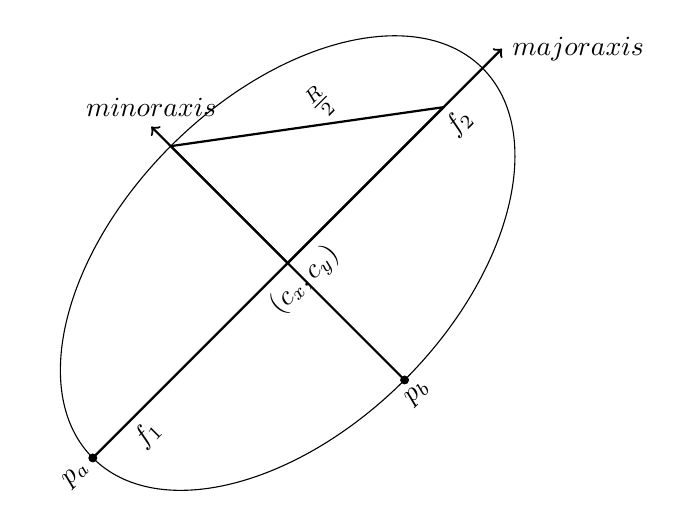
\begin{tikzpicture}[xscale=0.7, yscale=0.7][domain=0:11]
   % \draw [help axis] (-5,-3) grid (5,3);

    \begin{scope}[rotate=45]
    \draw (0,0) ellipse (5cm and 3cm);
    \node[rotate=45][below] at (-4,0) {$f_1$};
    \node[rotate=45][below] at (4,0) {$f_2$};
    \draw[fill] (-4,0) circle [radius=.5pt];
    \draw[fill] (4,0) circle [radius=.5pt];
    \draw [thick] (4,0) -- (0,0) -- (0,3) -- (4,0);
    \draw[->,thick] (-5,0)--(5.5,0) node[right]{$major axis$};
    \draw[->,thick] (0,-3)--(0,3.5) node[above]{$minor axis$};
        \node[rotate=45] [below] at (0,0) {$(c_x,c_y)$};
    \node [rotate=45][right] at (2.1,1.65) {$\frac{R}{2}$};
    
    \node [rotate=45][left] at (-5,0) {$p_a$};
    \draw[fill] (-5,0) circle [radius=2pt];
    
    \draw[fill] (0,-3) circle [radius=2pt];
    \node [below][rotate=45] at (0,-3) {$p_b$};
    \end{scope}

    %a^2-b^2=c^2 -> c^2=25-9=16 -> c=4
    
    %\draw[fill] (0,0) circle [radius=.5pt];
	
    %
    %\draw[fill] (5,0) circle [radius=1pt];
    %\draw[fill] (0,3) circle [radius=1pt];
    %
    

    %\node [below] at (2.1,0) {$c$};
	%\node [left] at (-0.1,1.5) {$b$};



    %\node [above] at (5,0) {$(x_0+a,y_0)$};
    %\node [above] at (-5,0) {$(x_0-a,y_0)$};
    %\node [above] at (0,3) {$(x_0,y_0+b)$};
    %
    

    
    %\draw [-] (-5,0) -- (5,0);
     %\draw [-] (0,-3) -- (0,3);
     %\draw [|-|] (0.001,-0.1) -- (4.999,-0.1);
\end{tikzpicture}
    \fautor
    \label{fig:ellipse_with_foci}
\end{figure}

Also, in \autoref{fig:ellipse_with_foci}, the distance $a = ||p_a - c||_2$, where $p_a$ is one of the intersection points of the ellipse with the major axis, is called the semi-major, and the distance $b = ||p_b-c||_2$, where $p_b$ is one of the intersection points of the ellipse with the minor axis, is called the semi-minor. These two values are also referred to as the shape parameters of an ellipse. Let $d = ||c-f_1||_2$, then it is easy to see that $a = R - d$ and $b = \sqrt{\frac{R^2}{4} - d^2}$.

Finally, an ellipse is said to be axis-parallel if its major-axis (see \autoref{fig:ellipse_with_foci}), which is the line that passes through its two foci points, is parallel to the $x$-axis.

\subsection{Axis-parallel}

An axis parallel ellipse centered at $c = (c_x,c_y)$ can be described using \autoref{def:ellipse} with $Q$ being a diagonal matrix \footnote{The only non-zero terms are in the main diagonal.}. This can be understood as a scaling transformation applied to the Euclidean norm.

Defining the matrix $Q$ as

\[
Q=
\left( {\begin{array}{cc}
    \frac{1}{a^2} & 0 \\
    0 & \frac{1}{b^2} \\
    \end{array} } \right),
\]

\noindent then, starting from \autoref{def:ellipse}, we can obtain the following equation

\begin{align*}
        (p-c)^{T}Q(p-c) = 1 & \Rightarrow \\
    (\frac{p_x-c_x}{a^2}, \frac{p_y-c_y}{b^2})^{T}(p_x-c_x, p_y-c_y) = 1 & \Rightarrow
 \end{align*}
 \begin{equation}\label{equation:pellipse}
  \frac{(p_x-c_x)^2}{a^2} + \frac{(p_y-c_y)^2}{b^2} = 1,
 \end{equation}

\noindent where $a$ and $b$ are the semi-major and semi-minor shape parameters, respectively.

Also, the coverage region is determined by just changing the equality to a inequality as follows

\begin{equation}\label{equation:cover_pellipse}
\frac{(p_x-c_x)^2}{a^2} + \frac{(p_y-c_y)^2}{b^2} \le 1.
\end{equation}

Another way to represent ellipses, which will be useful in some occasions, is through writing it as a curve, function of the angle with its major-axis (see \autoref{fig:ellipse_params}).

\begin{figure}[H]
    \centering
    
    \caption{The ellipse as a parametric curve.}
    

%\tikzset{every picture/.style={line width=0.75pt}} %set default line width to 0.75pt        

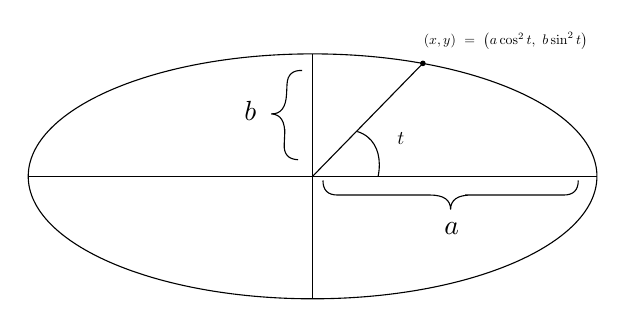
\begin{tikzpicture}[x=0.75pt,y=0.75pt,yscale=-1,xscale=1]
%uncomment if require: \path (0,300); %set diagram left start at 0, and has height of 300

%Shape: Ellipse [id:dp1559950964552308] 
\draw   (100,180) .. controls (100,147.42) and (161.34,121) .. (237,121) .. controls (312.66,121) and (374,147.42) .. (374,180) .. controls (374,212.58) and (312.66,239) .. (237,239) .. controls (161.34,239) and (100,212.58) .. (100,180) -- cycle ;
%Straight Lines [id:da3716259356733107] 
\draw    (100,180) -- (374,180) ;


%Straight Lines [id:da9880464900454329] 
\draw    (237,121) -- (237,239) ;


%Shape: Brace [id:dp3973633345998604] 
\draw   (242,182) .. controls (242,186.67) and (244.33,189) .. (249,189) -- (293.5,189) .. controls (300.17,189) and (303.5,191.33) .. (303.5,196) .. controls (303.5,191.33) and (306.83,189) .. (313.5,189)(310.5,189) -- (358,189) .. controls (362.67,189) and (365,186.67) .. (365,182) ;
%Shape: Brace [id:dp94498526835576] 
\draw   (232,129) .. controls (227.34,128.79) and (224.9,131.01) .. (224.68,135.67) -- (224.47,140.23) .. controls (224.16,146.89) and (221.68,150.11) .. (217.01,149.9) .. controls (221.68,150.11) and (223.85,153.55) .. (223.54,160.21)(223.68,157.21) -- (223.33,164.68) .. controls (223.12,169.35) and (225.34,171.79) .. (230,172) ;
%Shape: Arc [id:dp3154280429415799] 
\draw  [draw opacity=0] (258.54,158.43) .. controls (260.37,158.96) and (262.06,159.82) .. (263.54,161.03) .. controls (268.5,165.07) and (270.12,172.1) .. (268.62,179.79) -- (244.51,184.38) -- cycle ; \draw   (258.54,158.43) .. controls (260.37,158.96) and (262.06,159.82) .. (263.54,161.03) .. controls (268.5,165.07) and (270.12,172.1) .. (268.62,179.79) ;
%Shape: Circle [id:dp8908034615999807] 
\draw  [fill={rgb, 255:red, 0; green, 0; blue, 0 }  ,fill opacity=1 ] (289.08,125.57) .. controls (289.08,124.98) and (289.56,124.51) .. (290.14,124.51) .. controls (290.73,124.51) and (291.21,124.98) .. (291.21,125.57) .. controls (291.21,126.16) and (290.73,126.64) .. (290.14,126.64) .. controls (289.56,126.64) and (289.08,126.16) .. (289.08,125.57) -- cycle ;
%Straight Lines [id:da6323920079482996] 
\draw    (290.14,125.57) -- (237,180) ;



% Text Node
\draw (304,205) node   {$a$};
% Text Node
\draw (207,148.33) node   {$b$};
% Text Node
\draw (330,114.67) node [scale=0.5]  {$( x,y) \ =\ \left( a\cos^{2} t,\ b\sin^{2} t\right)$};
% Text Node
\draw (279.6,162) node [scale=0.7]  {$t$};


\end{tikzpicture}

    \fautor
    \label{fig:ellipse_params}
\end{figure}

Let $c \in \R^2$ be the center of an ellipse with shape parameters $(a,b) \in \R^2_{>0}$. Then $\gamma : [0, 2\pi] \mapsto \R^2$ defines a curve which maps every angle onto a point on the ellipse and it is defined as follows

    \begin{equation}\label{eq:parametric_ellipse}
    \gamma(t) = \left\{
    \begin{array}{l}
    x(t)= a\cos{t} + c_x,\\
    y(t)=b\sin{t} + c_y.
    \end{array}
    \right.
    \end{equation}

No equivalent disk-circle wording exists for ellipses, this could be a source of ambiguity in the text, that is why a note for the reader was judged to be necessary. Throughout this work an ellipse will represent the set of points that satisfy \autoref{def:ellipse}. In some places, though, with prior clarification, we will denote as an ellipse the set of points that are covered by the ellipse itself. For example, when we define $\Pp \cap E$ as the set of points in $\Pp$ that are covered by $E$, we are implicitly calling $E$ the set of points that are covered by the ellipse itself as it is defined by \autoref{def:ellipse}.